%% Blowup above the exponent one third in viscous Katz--Pavlovic dyadic models with small shell ratios
\documentclass[11pt,reqno]{amsart}

\usepackage[T1]{fontenc}
\usepackage{lmodern}
\usepackage{amsmath,amssymb,amsthm,mathtools}
\usepackage[kerning=true]{microtype}
\usepackage{enumitem}
\usepackage[margin=1.12in]{geometry}
\usepackage{booktabs,array}
\usepackage{graphicx}
\usepackage{xcolor}
\usepackage[colorlinks=true,linkcolor=blue!55!black,citecolor=blue!55!black,urlcolor=blue!55!black]{hyperref}

\numberwithin{equation}{section}
\raggedbottom

\theoremstyle{plain}
\newtheorem{theorem}{Theorem}[section]
\newtheorem{lemma}[theorem]{Lemma}
\newtheorem{proposition}[theorem]{Proposition}
\newtheorem{corollary}[theorem]{Corollary}
\newtheorem{conjecture}[theorem]{Conjecture}
\theoremstyle{definition}
\newtheorem{definition}[theorem]{Definition}
\theoremstyle{remark}
\newtheorem{remark}[theorem]{Remark}

\newcommand{\Kb}{K_{\mathrm b}}
\newcommand{\Ka}{K_{\mathrm a}}
\newcommand{\Glo}{G_{\mathrm{lo}}}
\newcommand{\Ghi}{G_{\mathrm{hi}}}
\newcommand{\send}{s_{\mathrm{end}}}
\newcommand{\Wd}{W_{\mathrm d}}
\newcommand{\R}{\mathbb{R}}
\newcommand{\N}{\mathbb{N}}
\newcommand{\eps}{\varepsilon}
%% Zenodo archive of the code; the concept DOI is added once the first release is minted.
\newcommand{\zenodoline}{}

\title[Blowup above one third in dyadic models]
{Blowup above the exponent one third in viscous Katz--Pavlovi\'c dyadic models with small shell ratios}

\author{Deep Bhattacharjee}
\address{Formerly, Electro-Gravitational Space Propulsion Laboratory (EGSPL),
  Bhubaneswar, Odisha 751030, India}
\email{d.bhattacharjee@erl-forschung.de}
\email{itsdeep@live.com}
\urladdr{\textnormal{ORCID
  \href{https://orcid.org/0000-0003-0466-750X}{0000-0003-0466-750X}}}

\subjclass[2020]{Primary 35Q30, 34A34; Secondary 35B44, 76F02, 65G30}
\keywords{dyadic model, Katz--Pavlovi\'c model, finite-time blowup,
dissipation exponent, self-similar front, computer-assisted proof}
\date{}

\begin{document}

\begin{abstract}
For the viscous Katz--Pavlovi\'c dyadic model with shell ratio
$\Lambda>2^{3/2}$, global regularity holds exactly for dissipation
exponents $\alpha\ge1/3$. We prove that this threshold is not universal:
for $\Lambda=6/5$, $13/10$, $3/2$, $17/10$ and $9/5$, suitable
nonnegative finitely supported data lose regularity in finite time for
every $\alpha\le\alpha_\Lambda$, where $\alpha_\Lambda>1/3$; for example
$\alpha_{13/10}=0.378$. The blowup is carried by a self-similar energy
front whose amplitude grows by a fixed factor $\kappa>1$ per shell. The
proof reduces the dynamics to one renormalized step of the front and
verifies that step in interval arithmetic.
\end{abstract}

\maketitle

\section{Introduction}\label{sec:intro}

\subsection{The model}
Fix a shell ratio $\Lambda>1$, a viscosity $\nu>0$ and a dissipation
exponent $\alpha$. The viscous Katz--Pavlovi\'c dyadic model is the
infinite system
\begin{equation}\label{eq:KP}
  \dot u_n+\nu\Lambda^{2\alpha n}u_n=\Lambda^{n-1}u_{n-1}^2-\Lambda^n u_nu_{n+1},
  \qquad n\ge0,\qquad u_{-1}\equiv0 .
\end{equation}
The coordinate $u_n$ models the velocity at frequency $\Lambda^n$; the
quadratic terms move energy from shell $n-1$ to shell $n$ and conserve
$\sum u_n^2$, and the linear term dissipates it. Katz and Pavlovi\'c
introduced the model for $\Lambda=2$ as a scalar caricature of the
Navier--Stokes nonlinearity \cite{KP05}; see \cite{FP04,Wal06,KZ05,CFP07,BFM11,Jeo19}
for related models and \cite{CDF23} for a survey. Writing the shells as
$N_n=N_0\Lambda^n$, as in \cite{Zha26}, changes only $\nu$: the substitution
$u\mapsto N_0u$ turns that system into \eqref{eq:KP} with viscosity
$\nu N_0^{2\alpha}$.

For $\sigma\ge0$ let $\|u\|_{H^\sigma}^2=\sum_{n\ge0}\Lambda^{2\sigma n}u_n^2$.
Following \cite{Che08,Zha26}, a \emph{finite-energy solution} on an interval
$I\ni0$ is an $\ell^2$-valued map whose coordinates are $C^1$ on $I$ and
satisfy \eqref{eq:KP}; it is \emph{smooth} on $I$ if
$\sup_{t\in J}\|u(t)\|_{H^\sigma}<\infty$ for every compact $J\subset I$
and every $\sigma>0$. A nonnegative datum in every $H^\sigma$ has a unique
nonnegative smooth solution on a maximal interval $[0,T_{\max})$
\cite[Remark~3.4]{BMR11}, \cite[Proposition~2.4]{Zha26}; it \emph{loses
regularity in finite time} if $T_{\max}<\infty$.

The known results on regularity are these. Katz and Pavlovi\'c proved
finite-time blowup for $\alpha<1/4$ \cite{KP05}. Cheskidov proved, for every
$\Lambda>1$, that large nonnegative data blow up in $H^{1/3+\gamma}$ when
$\alpha<1/3$, and that all solutions are regular when $\alpha\ge1/2$
\cite[Theorems~4.4 and~5.3]{Che08}. Barbato, Morandin and Romito proved
smoothing in an intermediate range \cite{BMR11}. Recently Zhang proved
global regularity of all nonnegative smooth data when
\begin{equation}\label{eq:Zhang}
  \alpha\ge\tfrac13\qquad\text{and}\qquad 4\alpha-1>\frac{\log2}{2\log\Lambda}
\end{equation}
\cite[Theorem~1.2]{Zha26}. For $\Lambda>2^{3/2}$ the second condition
follows from the first, so $\alpha=1/3$ is the sharp threshold for these
ratios. Zhang notes that the restriction on $\Lambda$ comes from the method
and does not assert that it is optimal. For $\Lambda\le2^{3/2}$ the range
between $1/3$ and $\min\{1/2,\,1/4+\log2/(8\log\Lambda)\}$ was open.

\subsection{Main result}
The theorem below shows that for small shell ratios the threshold lies
strictly above $1/3$. Table~\ref{tab:main} lists, for five ratios, the
window sizes $\Kb,\Ka$ of the computation, the exponent $\alpha_\Lambda$
reached, an enclosure $[\Glo,\Ghi]$ of the growth factor of the front, and
two constants $\gamma_\Lambda$ and $C_\Lambda$. For each row, $w^*=(w^*_k)_{-\Kb\le
k\le\Ka}$ is a profile with $w^*_0=1$, $w^*_1=1/2$, all $w^*_k\ge0$; its
values are stored to $17$ digits in the file
\texttt{cap/cases/center\_L*.txt} of the archive \cite{Data}, and
Table~\ref{tab:profile} shows part of the profile for $\Lambda=13/10$. Put
\begin{equation}\label{eq:datum}
  h^0_m=\Lambda^{-m/3}w^*_{m-\Kb}\quad(0\le m\le\Kb+\Ka),\qquad h^0_m=0\quad(m>\Kb+\Ka).
\end{equation}

\begin{table}[ht]
\centering\small
\caption{The five verified cases. $\alpha_\Lambda$ is the largest exponent
covered by the computation, $[\Glo,\Ghi]$ encloses the growth factor of
one step, $\gamma_\Lambda=1/3-\log\Glo/\log\Lambda$ and $C_\Lambda$ are
rounded up. The last column is $1/3+\log\Glo/(2\log\Lambda)$, the
largest exponent for which this $\Glo$ would close the argument.}
\label{tab:main}
\begin{tabular}{@{}lccclccc@{}}
\toprule
$\Lambda$ & $\Kb$ & $\Ka$ & $\alpha_\Lambda$ & \multicolumn{1}{c}{$[\Glo,\Ghi]$} & $\gamma_\Lambda$ & $C_\Lambda$ & $\tfrac13+\tfrac{\log\Glo}{2\log\Lambda}$\\
\midrule
$6/5$   & 80 & 7 & $0.377$ & $[1.01628489,\,1.01628532]$ & $0.24474$ & $2.83\cdot10^{-4}$ & $0.37763$\\
$13/10$ & 60 & 6 & $0.378$ & $[1.02401568,\,1.02401602]$ & $0.24288$ & $8.72\cdot10^{-5}$ & $0.37856$\\
$3/2$   & 50 & 8 & $0.365$ & $[1.02642827,\,1.02642851]$ & $0.26900$ & $2.82\cdot10^{-6}$ & $0.36550$\\
$17/10$ & 40 & 8 & $0.348$ & $[1.01599737,\,1.01599757]$ & $0.30343$ & $1.04\cdot10^{-6}$ & $0.34828$\\
$9/5$   & 40 & 8 & $0.339$ & $[1.00747733,\,1.00747753]$ & $0.32066$ & $2.02\cdot10^{-7}$ & $0.33967$\\
\bottomrule
\end{tabular}
\end{table}

\begin{theorem}\label{thm:main}
Let $(\Lambda,\Kb,\Ka,\alpha_\Lambda)$ be a row of Table~\ref{tab:main} and
let $h^0$ be the datum \eqref{eq:datum}. Let $\nu>0$, $0<\alpha\le\alpha_\Lambda$, and
\begin{equation}\label{eq:A0}
  A\ \ge\ A_0(\nu,\alpha):=10^{12}\,\nu\,\Lambda^{1/3}\,\Lambda^{(2\alpha-2/3)\Kb}.
\end{equation}
\begin{enumerate}[label=\textup{(\alph*)}]
\item Let $u$ be a nonnegative finite-energy solution of \eqref{eq:KP} on
  $[0,T)$ with $u(0)=Ah^0$ and $T>C_\Lambda/A$. There are times
  $0=t_{\Kb}<t_{\Kb+1}<\dotsb$ with $t_n<C_\Lambda/A$ such that
  \[
    u_n(t_n)\ \ge\ A\,\Lambda^{-n/3}\,\Glo^{\,n-\Kb}\qquad(n\ge\Kb).
  \]
  Consequently $\|u(t_n)\|_{H^\sigma}\to\infty$ for every
  $\sigma>\gamma_\Lambda$, and $u$ is not smooth on $[0,C_\Lambda/A]$.
\item The smooth solution with datum $Ah^0$ has $T_{\max}\le C_\Lambda/A$.
  More precisely, $T_{\max}=\lim_n t_n$.
\end{enumerate}
\end{theorem}

Nonnegative finite-energy solutions with any nonnegative $\ell^2$ datum
exist for all time \cite[Theorem~4.1]{Che08}, so part~(a) says that every
global such solution with datum $Ah^0$ loses $H^\sigma$ regularity, for
$\sigma>\gamma_\Lambda$, before the time $C_\Lambda/A$. Since $\alpha_\Lambda>1/3$ in
every row, we obtain:

\begin{corollary}\label{cor:threshold}
For $\Lambda\in\{6/5,\,13/10,\,3/2,\,17/10,\,9/5\}$ and every
$\alpha\in[1/3,\alpha_\Lambda]$, global regularity of \eqref{eq:KP} fails for some
nonnegative finitely supported datum. In particular, the condition
$\alpha\ge1/3$ alone does not imply global regularity, and the
restriction on $\Lambda$ in \eqref{eq:Zhang} cannot be dropped.
\end{corollary}

For $\Lambda=13/10$ the second condition in \eqref{eq:Zhang} requires
$\alpha>0.5802$, so the corollary is consistent with \cite{Zha26}; the
range $0.378<\alpha<1/2$ remains open for this ratio
(Figure~\ref{fig:phase}(b)).

\begin{remark}\label{rem:open}
The proof uses only that the front coordinates of the datum at shell
$\Kb$ satisfy (S1)--(S5) of Definition~\ref{def:S}. Hence the conclusions
hold for every datum $Ag$ with $g\ge0$, $g_m=\Lambda^{-m/3}v_{m-\Kb}$ for
$0\le m\le\Kb+\Ka$, where $v_0=1$, $v_1=1/2$ and the other $v_k$ lie in the
box $B$ of (S2), and with $g_m\le\Lambda^{-m/3}\theta_{m-\Kb}$ for $m>\Kb+\Ka$. These
data form a relatively open subset of a hyperplane; we have not checked
the step for states near the section but off it. The time $C_\Lambda/A$ scales like the
inverse amplitude; by the scaling $u\mapsto au(a\,\cdot)$, which maps
viscosity $\nu$ to $a\nu$, the theorem equivalently gives blowup of the
fixed datum $h^0$ for every viscosity $\nu\le10^{-12}\Lambda^{-1/3}\Lambda^{(2/3-2\alpha)\Kb}$.
\end{remark}

\subsection{The mechanism}
Set $y_n=\Lambda^{n/3}u_n$. Kolmogorov scaling corresponds to $y_n$ of order
one, and in these variables the inviscid model has the rate ratio
$r=\Lambda^{2/3}$ between neighbouring shells (Section~\ref{sec:front}). Energy
injected at low shells forms a front that moves to higher shells. After
the front has passed shell $n$, the profile seen from the front repeats
itself up to a factor: the amplitude of the leading shell grows by a
factor $\kappa(\Lambda)$ per shell, and the passage through shell $n$
takes a time proportional to $(r\kappa)^{-n}$. Viscosity at the front is
measured by $\eps_n\propto\Lambda^{2\alpha n}/(r\kappa)^{n}$, which tends to zero
when
\begin{equation}\label{eq:mech}
  \Lambda^{2\alpha}<r\kappa\qquad\Longleftrightarrow\qquad
  \alpha<\frac13+\frac{\log\kappa}{2\log\Lambda}.
\end{equation}
If $\kappa=1$, as for a front with Kolmogorov scaling, this is Cheskidov's
range $\alpha<1/3$. Numerically, $\kappa(\Lambda)>1$ exactly when
$\Lambda<\Lambda_c\approx1.8754$ (Section~\ref{sec:numerics} and
Figure~\ref{fig:phase}(a)). Then $y_n$ at the front grows like $\kappa^n$,
$u_n$ decays only like $\Lambda^{-\gamma n}$ with
$\gamma=1/3-\log\kappa/\log\Lambda<1/3$, and the window \eqref{eq:mech} extends
beyond $1/3$. Figure~\ref{fig:front} shows the front for $\Lambda=13/10$.

\begin{figure}[ht]
\centering
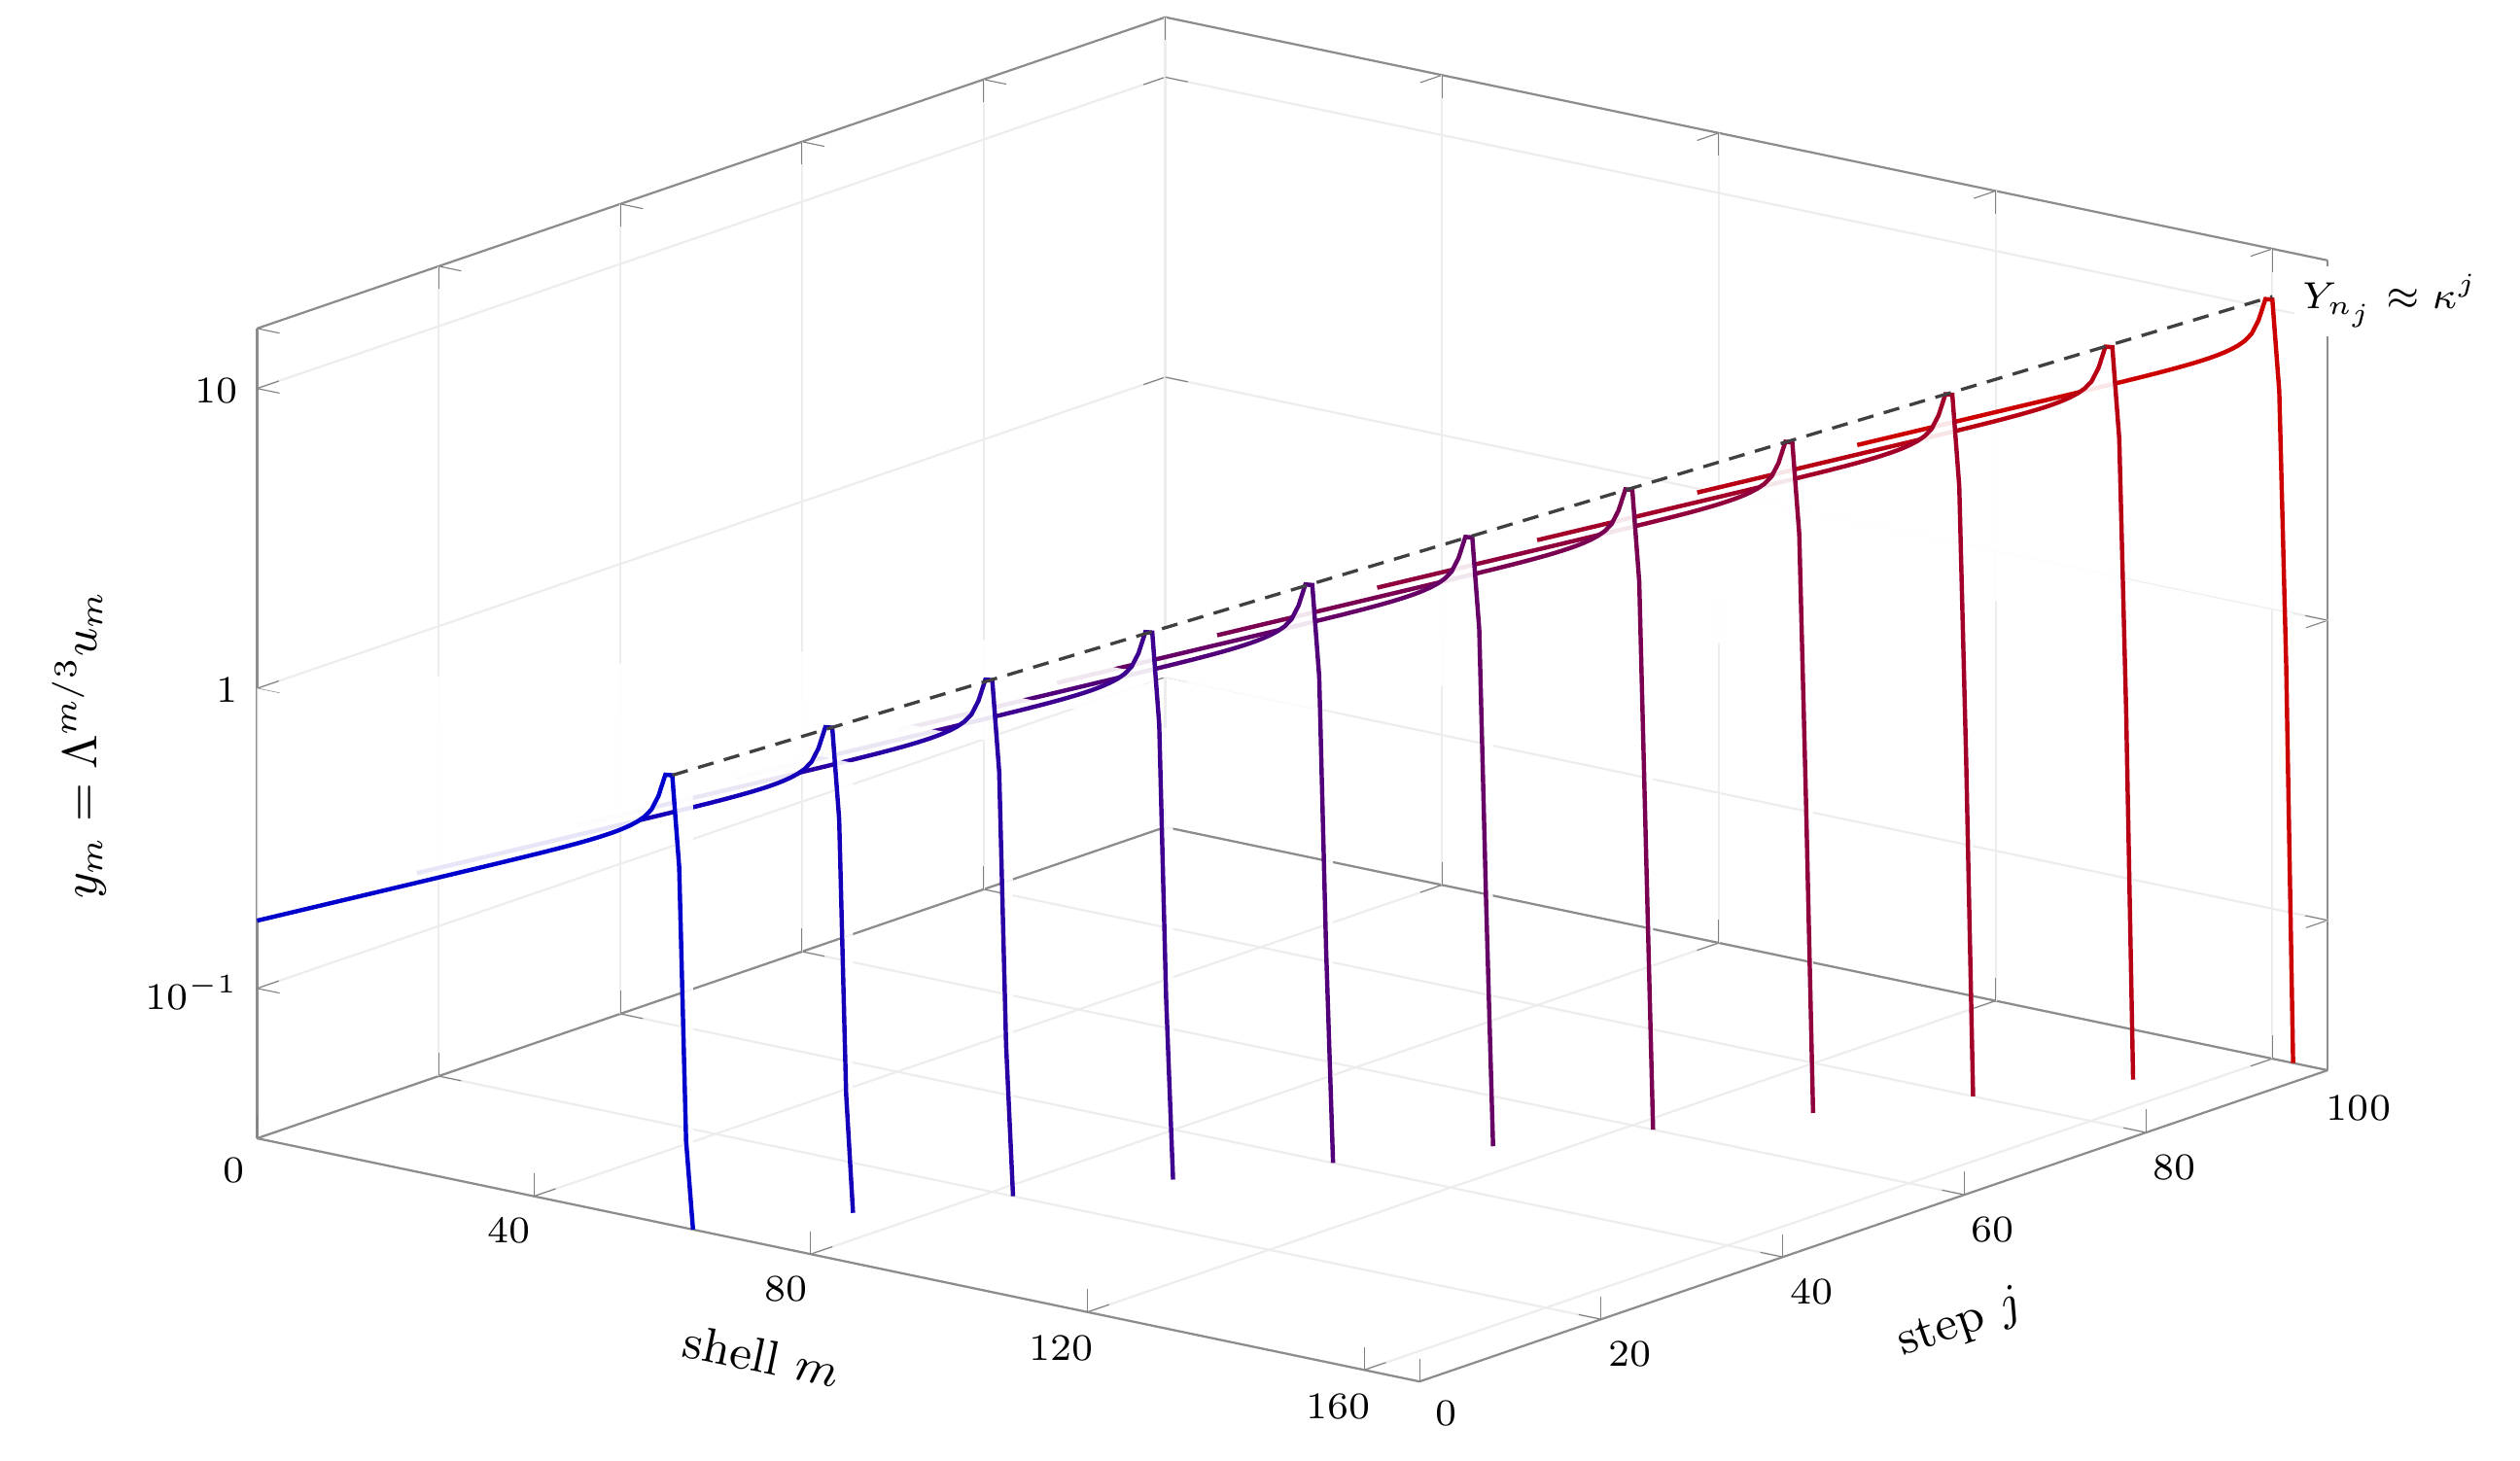
\includegraphics[width=0.94\textwidth]{figures/fig_front.png}
\caption{The front for $\Lambda=13/10$, $\alpha=3/8$: the compensated
amplitudes $y_m=\Lambda^{m/3}u_m$ at the start of every tenth renormalized
step $j$, computed from the datum $h^0$ (Section~\ref{sec:numerics}). Each
step moves the front by one shell and multiplies its height by
$\kappa\approx1.024016$; the dashed line has slope $\log_{10}\kappa$ per step.
Values below $10^{-1.5}$ are cut off.}
\label{fig:front}
\end{figure}

\subsection{Method and what the computer checks}\label{sec:method}
We write the solution in coordinates attached to the front
(Section~\ref{sec:front}) and show that one renormalized step maps a box $B$
of states into itself, with growth factor at least $\Glo>1$ and with the
viscosity parameter decreasing (Proposition~\ref{prop:step}). Iterating the
step proves Theorem~\ref{thm:main} (Section~\ref{sec:proof}).

The following parts are proved by hand: the reduction to front
coordinates (Lemmas~\ref{lem:scaling} and~\ref{lem:renorm}), the
iteration that gives Theorem~\ref{thm:main} from
Proposition~\ref{prop:step}, and the five lemmas of
Section~\ref{sec:lemmas} that control the infinitely many shells outside a
finite window, the error of truncating to that window, and the crossing
of the section. Eight of these elementary lemmas are also formalized in
Lean~4 (Appendix~\ref{app:code}).

What remains is a finite list of inequalities, (V1)--(V9) in
Section~\ref{sec:computation}, about one system of $\Kb+\Ka+1$ ordinary
differential equations with parameters $\eps\in[0,10^{-12}]$ and
$\alpha\in[0,\alpha_\Lambda]$. These are verified by a computer in interval
arithmetic with the CAPD library \cite{CAPD21,Zgl02}. The computation
encloses the flow of the truncated system over one step, together with
its derivative, for all states in $B$ at once. Thus the proof is
computer-assisted in the usual sense \cite{GS19}: it is rigorous provided
the CAPD library and our program, both public, are correct. Each case
takes a few seconds (Table~\ref{tab:verif}).

\subsection{Scope}
The result concerns the dyadic model, not the Navier--Stokes equations.
It shows that the threshold $1/3$, which matches the scaling of the
three-dimensional equations and is sharp for $\Lambda>2^{3/2}$, is an
artifact of the shell geometry for small $\Lambda$: there the front
develops anomalous scaling, and the dissipation needed to stop it is
larger. Section~\ref{sec:numerics} records the numerical picture for all
$\Lambda$ and a conjecture on the threshold; Section~\ref{sec:open} lists open
questions.

\section{Front coordinates}\label{sec:front}

Throughout, $u$ is a nonnegative finite-energy solution of \eqref{eq:KP} on
$[0,T)$, and $r=\Lambda^{2/3}$.

\begin{lemma}[Positivity]\label{lem:pos}
If $u(0)\ge0$ coordinatewise, then $u_n(t)\ge0$ for all $n$ and $t$.
\end{lemma}

\begin{proof}
Put $a_n(t)=\nu\Lambda^{2\alpha n}+\Lambda^nu_{n+1}(t)$, a continuous function. Then
\[
  \frac{d}{dt}\Bigl(u_ne^{\int_0^ta_n}\Bigr)=\Lambda^{n-1}u_{n-1}^2e^{\int_0^ta_n}\ge0,
\]
so $u_n(t)\ge u_n(0)e^{-\int_0^ta_n}\ge0$.
\end{proof}

\begin{lemma}[Scaling]\label{lem:scaling}
Let $y_n(\tau)=\Lambda^{n/3}u_n(\Lambda^{1/3}\tau)$ and $\tilde\nu=\Lambda^{1/3}\nu$. Then
\begin{equation}\label{eq:y}
  \frac{dy_n}{d\tau}=r^n\bigl(y_{n-1}^2-y_ny_{n+1}\bigr)-\tilde\nu\Lambda^{2\alpha n}y_n,
  \qquad y_{-1}\equiv0.
\end{equation}
\end{lemma}

\begin{proof}
With $t=\Lambda^{1/3}\tau$ and $u_m=\Lambda^{-m/3}y_m$,
\[
\frac{dy_n}{d\tau}=\Lambda^{1/3}\Lambda^{n/3}\Bigl(\Lambda^{n-1}\Lambda^{-2(n-1)/3}y_{n-1}^2
-\Lambda^{n}\Lambda^{-n/3-(n+1)/3}y_ny_{n+1}-\nu\Lambda^{2\alpha n}\Lambda^{-n/3}y_n\Bigr),
\]
and both quadratic coefficients equal $\Lambda^{2n/3}=r^n$.
\end{proof}

\begin{definition}[Front coordinates]\label{def:front}
Let $n\ge0$ and $\tau_n\in[0,\Lambda^{-1/3}T)$ with $Y_n:=y_n(\tau_n)>0$. The
\emph{front coordinates at $(n,\tau_n)$} are
\[
  Y_k(s)=\frac{y_{n+k}\bigl(\tau_n+s/(r^nY_n)\bigr)}{Y_n}\qquad(k\ge-n),
\]
the \emph{time of the step} is $s\ge0$, and the \emph{viscosity parameter} is
$\eps_n=\tilde\nu\Lambda^{2\alpha n}/(r^nY_n)$.
\end{definition}

The subscript of $Y_n$ refers to the shell and that of $Y_k$ to the
position relative to the front; no confusion will arise. Put
$R_k=r^k$ and $E_k=\eps_n\Lambda^{2\alpha k}$. Differentiating, and using
\eqref{eq:y} with $y_{n+k}=Y_nY_k$,
\begin{equation}\label{eq:front}
  \frac{dY_k}{ds}=R_k\bigl(Y_{k-1}^2-Y_kY_{k+1}\bigr)-E_kY_k\quad(k\ge-n),\qquad Y_{-n-1}\equiv0 .
\end{equation}
Indeed $\frac{dY_k}{ds}=\frac{1}{r^nY_n^2}\frac{dy_{n+k}}{d\tau}$, and
$\frac{1}{r^nY_n^2}\bigl(r^{n+k}Y_n^2(Y_{k-1}^2-Y_kY_{k+1})-\tilde\nu\Lambda^{2\alpha(n+k)}Y_nY_k\bigr)$
is the right side of \eqref{eq:front}. Fix $c=1/2$ and put
$h(Y)=Y_2-cY_1$.

\begin{lemma}[Renormalization]\label{lem:renorm}
Suppose that $Y_0(0)=1$, $Y_1(0)=c$, and that at some $s_*>0$ we have
$h(Y(s_*))=0$ and $G:=Y_1(s_*)>0$. Put $\tau_{n+1}=\tau_n+s_*/(r^nY_n)$. Then
$y_{n+1}(\tau_{n+1})=GY_n$, the front coordinates $Y'$ at $(n+1,\tau_{n+1})$ satisfy
\[
  Y'_k(0)=\frac{Y_{k+1}(s_*)}{G}\quad(k\ge-n-1),\qquad Y'_0(0)=1,\qquad Y'_1(0)=c,
\]
and $\eps_{n+1}=\eps_n\Lambda^{2\alpha}/(rG)$.
\end{lemma}

\begin{proof}
By definition $y_{n+1}(\tau_{n+1})=Y_nY_1(s_*)=GY_n$, and
$Y'_k(0)=y_{n+1+k}(\tau_{n+1})/(GY_n)=Y_{k+1}(s_*)/G$. In particular
$Y'_0(0)=1$ and $Y'_1(0)=Y_2(s_*)/G=cY_1(s_*)/G=c$. Finally
$\eps_{n+1}=\tilde\nu\Lambda^{2\alpha(n+1)}/(r^{n+1}GY_n)=\eps_n\Lambda^{2\alpha}/(rG)$.
\end{proof}

We call $Y_{-n},\dots,Y_{-\Kb-1}$ the \emph{deep tail}, $Y_{-\Kb},\dots,Y_{\Ka}$ the
\emph{window} and $Y_{\Ka+1},Y_{\Ka+2},\dots$ the \emph{ahead tail}. The deep tail is
empty when $n=\Kb$.

\begin{definition}[Admissible states]\label{def:S}
Fix a row of Table~\ref{tab:main} with profile $w^*$ and the radii
$\rho_k>0$ stored in \texttt{cap/cases/radii\_L*.txt} \cite{Data}. Let
$\Wd=1$, $\theta=10^{-31}$, $\theta_k=\theta\,2^{-(k-\Ka-1)}$ for $k>\Ka$, and
$\eps_0=10^{-12}$. For $n\ge\Kb$, the set $\mathcal S_n$ consists of the pairs
$(Y,\eps)$, $Y=(Y_k)_{k\ge-n}$, with
\begin{enumerate}[label=\textup{(S\arabic*)}]
\item $Y_k\ge0$ for all $k$, $Y_0=1$ and $Y_1=c$;
\item $|Y_k-w^*_k|<\rho_k$ for $-\Kb\le k\le\Ka$, $k\notin\{0,1\}$;
\item $Y_k\le\Wd$ for $-n\le k<-\Kb$;
\item $Y_k\le\theta_k$ for $k>\Ka$;
\item $0\le\eps\le\eps_0$.
\end{enumerate}
We write $B$ for the open box in (S2).
\end{definition}

\section{The step proposition and the proof of the theorem}\label{sec:proof}

\begin{proposition}[One step]\label{prop:step}
Fix a row of Table~\ref{tab:main}, let $0\le\alpha\le\alpha_\Lambda$, $n\ge\Kb$, and let
$\send$ be the number in Table~\ref{tab:verif}. Let $Y$ be a nonnegative
solution of \eqref{eq:front}, with coordinates of class $C^1$, on an
interval $[0,s_1]$, with $(Y(0),\eps_n)\in\mathcal S_n$.
\begin{enumerate}[label=\textup{(\roman*)}]
\item If $s_1\ge\send$, then $h(Y(s))$ has exactly one zero $s_*$ in
  $[0,\send]$; it is negative on $[0,s_*)$ and positive on $(s_*,\send]$.
\item In that case $G=Y_1(s_*)\in[\Glo,\Ghi]$, and the state
  $\bigl((Y_{k+1}(s_*)/G)_{k\ge-n-1},\ \eps_n\Lambda^{2\alpha}/(rG)\bigr)$
  lies in $\mathcal S_{n+1}$.
\item For every $s_1\le\send$, the coordinates satisfy on $[0,s_1]$
  \[
    Y_k\le\frac{\Wd}{1-\Wd R_{-\Kb-1}\send}\ (k<-\Kb),\quad Y_k\le M\ (|k|\le\Kb+\Ka),\quad Y_k\le2\theta_k\ (k>\Ka),
  \]
  with a constant $M$ depending only on the row.
\end{enumerate}
\end{proposition}

The proof of Proposition~\ref{prop:step} occupies
Sections~\ref{sec:lemmas} and~\ref{sec:computation}. We now derive
Theorem~\ref{thm:main}.

\begin{proof}[Proof of Theorem~\ref{thm:main}]
(a) Let $y,\tau$ be as in Lemma~\ref{lem:scaling}, and $T'=\Lambda^{-1/3}T$.
Put $n_0=\Kb$, $\tau_{n_0}=0$, $Y_{n_0}=y_{\Kb}(0)=A$. The front coordinates at
$(n_0,0)$ are $Y_k(0)=w^*_k$ for $-\Kb\le k\le\Ka$ and $Y_k(0)=0$ for $k>\Ka$, and
the deep tail is empty. By \eqref{eq:A0},
\[
  \eps_{n_0}=\frac{\tilde\nu\Lambda^{2\alpha\Kb}}{r^{\Kb}A}
  =\frac{\nu\Lambda^{1/3}\Lambda^{(2\alpha-2/3)\Kb}}{A}\le10^{-12},
\]
so $(Y(0),\eps_{n_0})\in\mathcal S_{n_0}$ (the profile has $w^*\ge0$ and lies in
$B$).

Let $D_\Lambda=\send/(r^{n_0}A)\sum_{i\ge0}(r\Glo)^{-i}$. We show by induction on
$n\ge n_0$: there are times $\tau_{n_0}<\dots<\tau_n$ with
\begin{equation}\label{eq:induction}
  \tau_n+\frac{\send}{r^nY_n}\le\sum_{j=n_0}^{n}\frac{\send}{r^jY_j}\le D_\Lambda,\qquad
  Y_j\ge A\Glo^{\,j-n_0},
\end{equation}
where $Y_j=y_j(\tau_j)$, and the front coordinates at $(n,\tau_n)$, together
with $\eps_n$, lie in $\mathcal S_n$. For $n=n_0$ this was shown. Assume it for
$n$. Since $\Lambda^{1/3}D_\Lambda=C_\Lambda/A<T$ (the value of $C_\Lambda$ in
Table~\ref{tab:main} is $\Lambda^{1/3}\send r^{-\Kb}(1-(r\Glo)^{-1})^{-1}$ rounded
up), the solution exists on $[\tau_n,\tau_n+\send/(r^nY_n)]$, so the front
coordinates solve \eqref{eq:front} on $[0,\send]$. Proposition~\ref{prop:step}
gives $s_*\le\send$ and $G\ge\Glo$, and Lemma~\ref{lem:renorm} gives
$\tau_{n+1}=\tau_n+s_*/(r^nY_n)$, $Y_{n+1}=GY_n\ge A\Glo^{\,n+1-n_0}$ and an admissible
state at $n+1$. Then
$\tau_{n+1}+\send/(r^{n+1}Y_{n+1})\le\sum_{j=n_0}^{n+1}\send/(r^jY_j)$, and the sum is at
most $\send r^{-n_0}A^{-1}\sum_{i\ge0}(r\Glo)^{-i}=D_\Lambda$.

Put $t_n=\Lambda^{1/3}\tau_n<C_\Lambda/A$. Then
$u_n(t_n)=\Lambda^{-n/3}Y_n\ge A\Lambda^{-n/3}\Glo^{\,n-\Kb}$ and
\[
  \|u(t_n)\|_{H^\sigma}\ge\Lambda^{\sigma n}u_n(t_n)\ge A\,\Glo^{-\Kb}\bigl(\Lambda^{\sigma-1/3}\Glo\bigr)^n,
\]
which tends to infinity when $\Lambda^{\sigma-1/3}\Glo>1$, that is,
$\sigma>1/3-\log\Glo/\log\Lambda$; Table~\ref{tab:main} lists this number rounded up.
Since all $t_n$ lie in $[0,C_\Lambda/A]$, $u$ is not smooth there.

(b) The smooth solution is a nonnegative finite-energy solution on
$[0,T_{\max})$. If $T_{\max}>C_\Lambda/A$, it would be smooth on $[0,C_\Lambda/A]$,
contradicting (a). Hence $T_{\max}\le C_\Lambda/A<\infty$.

Now run the induction of (a) for this solution, with $T=T_{\max}$; step $n$
can be carried out if $t_n+\Lambda^{1/3}\send/(r^nY_n)<T_{\max}$. Suppose that this
fails at some $n$. For every $t\in[t_n,T_{\max})$ the front coordinates at
$(n,\tau_n)$ solve \eqref{eq:front} on an interval $[0,s_1]$ with $s_1<\send$
that reaches the time $t$, and the state at $s=0$ is admissible. By
Proposition~\ref{prop:step}(iii), with $M'=\max\{M,\Wd/(1-\Wd R_{-\Kb-1}\send)\}$,
we get $y_{n+k}(\tau)\le M'Y_n$ for $k\le\Ka$ and
$y_{n+k}(\tau)\le2\theta_kY_n$ for $k>\Ka$, at the corresponding $\tau$. With
$\Lambda^mu_m=\Lambda^{2m/3}y_m$ and $\theta_k=2\theta\,2^{-(k-\Ka)}$ this gives
\[
  \sup_m\Lambda^mu_m(t)\le Y_n\Lambda^{2(n+\Ka)/3}\max\Bigl\{M',\,4\theta\sup_{j\ge1}\bigl(\Lambda^{2/3}/2\bigr)^{j}\Bigr\}
  \qquad(t_n\le t<T_{\max}),
\]
which is finite because $\Lambda^{2/3}<2$ for all five ratios. On the compact
interval $[0,t_n]$ the solution is smooth, so $\sup_m\Lambda^mu_m\le\|u\|_{H^1}$ is
bounded there too. This contradicts the continuation criterion of
\cite[Proposition~2.4]{Zha26}: if $T_{\max}<\infty$, then
$\limsup_{t\uparrow T_{\max}}\sup_m\Lambda^{qm}u_m(t)=\infty$ for every
$q>\max\{0,1-2\alpha\}$, in particular for $q=1$.

Hence every step is carried out, all $t_n<T_{\max}$, and $t_*:=\lim_nt_n\le T_{\max}$.
If $t_*<T_{\max}$, the solution would be smooth on the compact interval
$[0,t_*]$, which contains all $t_n$, whereas $\|u(t_n)\|_{H^\sigma}\to\infty$ by (a).
Hence $T_{\max}=t_*$.
\end{proof}

\begin{remark}
The proof of part (a) uses neither the energy inequality nor the local
theory; part (b) uses the local theory only through the existence of
the smooth solution and, for the identity $T_{\max}=\lim t_n$, through the
continuation criterion.
\end{remark}

\section{Lemmas for one step}\label{sec:lemmas}

Fix a row of Table~\ref{tab:main}, $\alpha\in[0,\alpha_\Lambda]$, $n\ge\Kb$, and a solution
$Y$ of \eqref{eq:front} on $[0,s_1]$ as in Proposition~\ref{prop:step}, with
$s_1\le\send$. The window $Z=(Y_k)_{-\Kb\le k\le\Ka}\in\R^{W}$, $W=\{-\Kb,\dots,\Ka\}$,
satisfies
\begin{equation}\label{eq:window}
  Z'=F(Z)+e(s),
\end{equation}
where $F$ is the right side of \eqref{eq:front} on the window with
$Y_{-\Kb-1}$ and $Y_{\Ka+1}$ replaced by $0$ (the \emph{truncated system}), and
the \emph{truncation error} $e$ has only two nonzero coordinates,
\begin{equation}\label{eq:e}
  e_{-\Kb}=R_{-\Kb}Y_{-\Kb-1}^2\ge0,\qquad e_{\Ka}=-R_{\Ka}Y_{\Ka}Y_{\Ka+1}\le0
\end{equation}
($e_{-\Kb}=0$ if $n=\Kb$). Since $\Ka\ge3$, the coordinates $e_1,e_2$ vanish,
so $h=Z_2-cZ_1$ has the same derivative $F_2-cF_1$ along \eqref{eq:window}
and along the truncated system. All coordinates are nonnegative by
Lemma~\ref{lem:pos}, which applies to \eqref{eq:front} by the same proof.
We write $\tilde Z$ for the solution of the truncated system $\tilde Z'=F(\tilde Z)$
with $\tilde Z(0)=Z(0)$.

\begin{lemma}[Deep tail]\label{lem:deep}
Let $\bar R=R_{-\Kb-1}$ and suppose $\Wd\bar R\send<1$ and $Y_k(0)\le\Wd$ for
$k<-\Kb$. Then $Y_k(s)\le\widehat W(s):=\Wd/(1-\Wd\bar Rs)$ for $-n\le k<-\Kb$ and
$s\in[0,s_1]$.
\end{lemma}

\begin{proof}
For $k<-\Kb$ we have $R_k\le\bar R$ and, dropping nonpositive terms,
$Y_k'\le\bar RY_{k-1}^2$, where $Y_{k-1}$ is a deep-tail coordinate or
$Y_{-n-1}=0$. For $\delta>0$ let
$B_\delta(s)=(\Wd+\delta)/(1-(\Wd+\delta)(\bar R+\delta)s)$ on the interval where the
denominator is positive; $B_\delta'=(\bar R+\delta)B_\delta^2$. If some $Y_k$ reaches
$B_\delta$, let $s_2$ be the first time at which $\max_{k<-\Kb}(Y_k-B_\delta)=0$ (a
maximum of finitely many continuous functions, negative at $s=0$), and
$k$ an index attaining it. Then $(Y_k-B_\delta)'(s_2)\ge0$, while
$Y_k'(s_2)\le\bar RY_{k-1}(s_2)^2\le\bar RB_\delta(s_2)^2<B_\delta'(s_2)$. Hence
$Y_k<B_\delta$ on the common interval, and letting $\delta\to0$ proves the claim.
\end{proof}

\begin{lemma}[Ahead tail]\label{lem:ahead}
Let $q_{\Ka}\ge\sup_{[0,s_1]}Y_{\Ka}$, put $q_{\Ka+1}=\theta+R_{\Ka+1}\send q_{\Ka}^2$ and
$q_k=\theta_k+R_k\send q_{k-1}^2$ for $k\ge\Ka+2$, and suppose $Y_k(0)\le\theta_k$ for
$k>\Ka$.
\begin{enumerate}[label=\textup{(\alph*)}]
\item $Y_k(s)\le q_k$ for all $k>\Ka$ and $s\in[0,s_1]$.
\item Suppose \textup{(A1)} $R_{\Ka+1}\send q_{\Ka}^2\le\theta$, \textup{(A2)} $r\le2$,
\textup{(A3)} $c_1:=4R_{\Ka+2}\send\theta\le1/2$, and \textup{(A4)} $1/2+c_1\le G_*$
for some $G_*>0$. Then $q_k\le2\theta_k$ for all $k>\Ka$, and
$q_k\le G_*\theta_{k-1}$ for all $k\ge\Ka+2$.
\end{enumerate}
\end{lemma}

\begin{proof}
(a) By induction on $k$: $Y_k'\le R_kY_{k-1}^2$, so
$Y_k(s)\le Y_k(0)+R_k\int_0^sY_{k-1}^2\le\theta_k+R_k\send q_{k-1}^2$.

(b) Write $a_k=4R_k\send\theta_{k-1}$ for $k\ge\Ka+2$; then $a_{\Ka+2}=c_1$ and
$a_{k+1}/a_k=r/2\le1$, so $a_k\le c_1\le1/2$. First,
$q_{\Ka+1}\le2\theta=2\theta_{\Ka+1}$ by (A1). If $q_{k-1}\le2\theta_{k-1}$, then, as
$\theta_k=\theta_{k-1}/2$,
\[
  q_k\le\theta_k+4R_k\send\theta_{k-1}^2=\theta_{k-1}\bigl(\tfrac12+a_k\bigr),
\]
which is at most $\theta_{k-1}=2\theta_k$ because $a_k\le1/2$, and at most
$G_*\theta_{k-1}$ because $1/2+a_k\le1/2+c_1\le G_*$.
\end{proof}

\begin{lemma}[Truncation error]\label{lem:comparison}
Let $H\subset\R^W$ be a box containing $\tilde Z(s)$ for $s\in[0,s_1]$, let
$D\in\R^W$ have positive entries, and let $M$ be a matrix with
\[
  M_{ii}\ge\sup\partial_iF_i,\qquad M_{ij}\ge\sup|\partial_jF_i|\ (i\ne j),
\]
the suprema taken over $H+[-D,D]$ and over the parameters. Let $\zeta\in\R^W$
have positive entries and $\lambda>0$ satisfy $M\zeta\le\lambda\zeta$. Let $\bar e\in\R^W$
satisfy $|e(s)|\le\bar e$ at every $s\in[0,s_1]$ such that $|Z-\tilde Z|\le D$ on
$[0,s]$, and let $\eta\ge0$ with $\bar e\le\eta\zeta$. If
$z:=\eta\zeta\,(e^{\lambda\send}-1)/\lambda<D$, then
\[
  |Z(s)-\tilde Z(s)|\le\eta\zeta\,\frac{e^{\lambda s}-1}{\lambda}\le z\qquad(0\le s\le s_1).
\]
All inequalities between vectors are coordinatewise.
\end{lemma}

This is the usual comparison argument for quasimonotone systems
\cite{Wal70}; we include the proof because the error bound $\bar e$ is
only available while $|Z-\tilde Z|\le D$.

\begin{proof}
Let $d=Z-\tilde Z$ and $s_2=\sup\{s\in[0,s_1]:|d|\le D\text{ on }[0,s]\}$; $s_2>0$
because $d(0)=0$. On $[0,s_2]$ both $Z$ and $\tilde Z$ lie in the convex box
$H+[-D,D]$, so $d'=A(s)d+e(s)$ with $A(s)=\int_0^1DF(\tilde Z+\vartheta d)\,d\vartheta$,
$A_{ii}\le M_{ii}$, $|A_{ij}|\le M_{ij}$ for $i\ne j$, and $|e|\le\bar e$.

For $\delta>0$ put $w^\delta(s)=\eta\zeta(e^{\lambda s}-1)/\lambda+\delta e^{(\lambda+1)s}\zeta$. We claim
$|d_i|<w^\delta_i$ on $[0,s_2]$ for all $i$. This holds at $s=0$. Otherwise
let $s_3$ be the first time with $|d_i(s_3)|=w^\delta_i(s_3)$ for some $i$. Then
$d_i(s_3)\ne0$, the function $|d_i|-w^\delta_i$ is differentiable at $s_3$,
negative before and zero at $s_3$, so its derivative there is $\ge0$. But
\[
  |d_i|'=\operatorname{sgn}(d_i)\,d_i'\le A_{ii}|d_i|+\sum_{j\ne i}|A_{ij}||d_j|+|e_i|
  \le(Mw^\delta)_i+\bar e_i,
\]
using $|d_j|\le w^\delta_j$ and $M_{ij}\ge0$ for $j\ne i$. Since $M\zeta\le\lambda\zeta$ and
$\bar e\le\eta\zeta$,
\[
  (Mw^\delta)_i+\bar e_i\le\eta(e^{\lambda s}-1)\zeta_i+\delta\lambda e^{(\lambda+1)s}\zeta_i+\eta\zeta_i
  <\eta e^{\lambda s}\zeta_i+\delta(\lambda+1)e^{(\lambda+1)s}\zeta_i=(w^\delta_i)'(s)
\]
at $s=s_3$, a contradiction. Letting $\delta\to0$ gives $|d|\le w^0\le z$ on $[0,s_2]$.
As $z<D$, continuity shows that $s_2<s_1$ is impossible.
\end{proof}

\begin{lemma}[Section crossing]\label{lem:section}
Let $0=\sigma_0<\sigma_1<\dots<\sigma_J=\send$ and let $E_j$ be boxes with
$\tilde Z(s)\in E_j$ for $s\in[\sigma_j,\sigma_{j+1}]$, for every initial state in $B$.
Let $z\ge0$ bound $|Z-\tilde Z|$ on $[0,\send]$ and put $E_j^z=E_j+[-z,z]$,
$\xi=z_2+cz_1$. Suppose that $h<0$ on $\bar B$, that for every $j$ either $h<0$ on $E_j^z$, or
$\nabla h\cdot F\ge m$ on $E_j^z$ for a constant $m>0$, and that $h>\xi$ on an
enclosure $E_{\mathrm{end}}$ of $\tilde Z(\send)$. Then:
\begin{enumerate}[label=\textup{(\alph*)}]
\item $h(\tilde Z(\cdot))$ and $h(Z(\cdot))$ each have exactly one zero in
  $[0,\send]$, at $\tilde s$ and $s_*$, are negative before it and positive after;
\item $|s_*-\tilde s|\le\xi/m$;
\item $|Z(s_*)-\tilde Z(\tilde s)|\le z+\bar F\xi/m$, where $\bar F$ bounds $|F+e|$ on
  the boxes $E_j^z$ of the second kind.
\end{enumerate}
\end{lemma}

\begin{proof}
Let $X$ be $\tilde Z$ or $Z$; then $X(s)\in E_j^z$ for $s\in[\sigma_j,\sigma_{j+1}]$, and
$\frac{d}{ds}h(X)=\nabla h\cdot F(X)$ because $e_1=e_2=0$. Whenever $h(X(s))\ge0$,
the box containing $X(s)$ is of the second kind, so $\frac{d}{ds}h(X)\ge m$.
Hence once $h(X)\ge0$ it increases strictly. Since $h(X(0))<0$ (both
start at the same point of $\bar B$) and $h(X(\send))>0$ (for $X=Z$ because
$|h(Z)-h(\tilde Z)|\le\xi$), there is exactly one zero, which proves (a). On the interval between
$\tilde s$ and $s_*$ the function $h(Z)$ is $\ge0$ (if $s_*<\tilde s$) or $h(\tilde Z)$ is
$\ge0$ (if $\tilde s<s_*$), so all boxes met there are of the second kind and
$\frac{d}{ds}h(Z)\ge m$ on it. Since $|h(Z(\tilde s))|=|h(Z(\tilde s))-h(\tilde Z(\tilde s))|\le\xi$,
the mean value theorem gives (b). For (c) write
$Z(s_*)-\tilde Z(\tilde s)=(Z(s_*)-Z(\tilde s))+(Z(\tilde s)-\tilde Z(\tilde s))$ and bound the first
term by $\bar F|s_*-\tilde s|$.
\end{proof}

\begin{lemma}[Image of the box]\label{lem:image}
For $P\in\R^W$ with $P_1>0$ let $\Phi(P)_k=P_{k+1}/P_1$ for $-\Kb\le k<\Ka$ and
$\Phi(P)_{\Ka}=0$. Let $\mathcal P\subset\R^W$ be a box with $P_1>0$ on $\mathcal P$,
containing $Z(s_*)$ and $\tilde Z(\tilde s)$. Then
\[
  \Phi(Z(s_*))\in\Phi(\tilde Z(\tilde s))+D\Phi(\mathcal P)\bigl(Z(s_*)-\tilde Z(\tilde s)\bigr),
\]
where $D\Phi(\mathcal P)$ is any interval matrix enclosing the Jacobian of $\Phi$ on $\mathcal P$,
and the renormalized window of Lemma~\ref{lem:renorm} equals
$\Phi(Z(s_*))+\bigl(0,\dots,0,Y_{\Ka+1}(s_*)/G\bigr)$.
\end{lemma}

\begin{proof}
The first claim is the mean value theorem applied coordinatewise on the
segment from $\tilde Z(\tilde s)$ to $Z(s_*)$, which lies in $\mathcal P$. The second is
Lemma~\ref{lem:renorm}: the renormalized window coordinate $k<\Ka$ is
$Y_{k+1}(s_*)/G=\Phi(Z(s_*))_k$, and coordinate $\Ka$ is $Y_{\Ka+1}(s_*)/G$.
\end{proof}

\section{The computation}\label{sec:computation}

\subsection{What is computed}
For each row of Table~\ref{tab:main} the program \texttt{cap/verify\_step.cpp}
\cite{Data} works with the truncated system on the window, with the
parameters $\eps\in[0,\eps_0]$ and $\alpha\in[0,\alpha_\Lambda]$ entering as intervals, and
with the box $\bar B$ (the closure of $B$, with $Z_0=1$, $Z_1=c$). All numbers
are intervals with outward rounding. It computes:
\begin{enumerate}[label=\textup{(C\arabic*)}]
\item an enclosure $\mathcal P_0$ of the first crossing point $\tilde Z(\tilde s)$ of the
  section $\{h=0\}$ from $\{h<0\}$, for all initial states in $\bar B$, with
  an enclosure of $\tilde s$, and an enclosure of the derivative of this
  Poincar\'e map; from the derivative and the image of the centre it
  forms the mean value enclosure and intersects it with $\mathcal P_0$;
\item boxes $E_j$ enclosing $\tilde Z$ on time intervals covering $[0,\send]$, with
  $\send=\sup\tilde s+0.02$ ($0.05$ for $\Lambda=3/2$), and an enclosure
  $E_{\mathrm{end}}$ of $\tilde Z(\send)$; $H$ is the hull of the $E_j$ and of $\bar B$.
\end{enumerate}
These use the $C^1$ Lohner algorithm of CAPD with Taylor order $20$
\cite{CAPD21,Zgl02}. It then checks:
\begin{enumerate}[label=\textup{(V\arabic*)}]
\item $\Wd R_{-\Kb-1}\send<1$; put $\widehat W=\Wd/(1-\Wd R_{-\Kb-1}\send)$.
\item The hypotheses of Lemma~\ref{lem:comparison} with $\bar e_{-\Kb}=R_{-\Kb}\widehat W^2$,
  $\bar e_{\Ka}=R_{\Ka}q_{\Ka}q_{\Ka+1}$, $\bar e_k=0$ otherwise, where $q_{\Ka}$ bounds
  $Z_{\Ka}$ on $H+[-D,D]$ and $q_{\Ka+1}$ is as in Lemma~\ref{lem:ahead}; the vector
  $D$ is found by iterating $D\leftarrow2z$, and the check is the strict
  inequality $z<D$.
\item The hypotheses of Lemma~\ref{lem:section}: $h<0$ on $\bar B$, the sign or
  slope condition on every $E_j^z$, and $h>\xi$ on $E_{\mathrm{end}}$.
\item With $\mathcal P=\mathcal P_0+[-1,1](z+\bar F\xi/m)$ and $\Glo=\inf_{\mathcal P}P_1$:
  conditions (A1)--(A4) of Lemma~\ref{lem:ahead} with $G_*=\Glo$.
\item $\Glo>1$ and $\Ghi=\sup_{\mathcal P}P_1$ (the values of Table~\ref{tab:main}).
\item For every $k\in W\setminus\{0,1\}$, the enclosure of the renormalized
  coordinate $k$ given by Lemma~\ref{lem:image}, with $[0,q_{\Ka+1}/\Glo]$ added
  at $k=\Ka$, lies in $(w^*_k-\rho_k,\,w^*_k+\rho_k)$.
\item $\sup_{\mathcal P}P_{-\Kb}/\Glo\le\Wd$ and $\widehat W/\Glo\le\Wd$.
\item $\Lambda^{2\alpha_\Lambda}/(r\Glo)<1$.
\item The mean value enclosure in (C1) and its intersection are nonempty
  (a consistency check).
\end{enumerate}

\begin{proof}[Proof of Proposition~\ref{prop:step}, given \textup{(V1)--(V9)}]
Lemma~\ref{lem:deep} applies by (V1) and (S3), and gives $e_{-\Kb}\le\bar
e_{-\Kb}$. While $|Z-\tilde Z|\le D$, the window coordinate $Z_{\Ka}$ is at most
$q_{\Ka}$, so Lemma~\ref{lem:ahead}(a) gives $Y_{\Ka+1}\le q_{\Ka+1}$ and
$|e_{\Ka}|\le\bar e_{\Ka}$. Lemma~\ref{lem:comparison} with (V2) gives $|Z-\tilde Z|\le z$
on $[0,s_1]$, hence $Z$ stays in $H+[-z,z]$ and $q_{\Ka}$ bounds $Z_{\Ka}$ on all of
$[0,s_1]$; with Lemma~\ref{lem:ahead}(b) under (V4) this proves (iii), with
$M=\sup(H+[-z,z])$. Now let $s_1\ge\send$. Lemma~\ref{lem:section} with (V3)
gives (i) and $Z(s_*)\in\mathcal P$, so $G=Z_1(s_*)\in[\Glo,\Ghi]$. The new state
satisfies (S1) by Lemma~\ref{lem:renorm} and positivity, (S2) by
Lemma~\ref{lem:image} and (V6), (S3) by (V7) (the new deep tail consists
of the old deep tail and the old coordinate $-\Kb$, divided by $G$), (S4)
by Lemma~\ref{lem:ahead}(b), since the new coordinate $k>\Ka$ is
$Y_{k+1}(s_*)/G\le q_{k+1}/\Glo\le\theta_k$, and (S5) by (V8), since
$\eps_n\Lambda^{2\alpha}/(rG)\le\eps_n\Lambda^{2\alpha_\Lambda}/(r\Glo)<\eps_n$.
\end{proof}

\subsection{The box}
Nothing in the choice of $w^*$ and $\rho$ needs to be rigorous. The profile
$w^*$ is the fixed point of the inviscid step map, found by iterating
the map on the truncated system with a high-order Runge--Kutta method.
The radii are
$\rho=\delta(I-|J|/0.9)^{-1}b$, where $J$ is the Jacobian of the step map at
$w^*$ (the program's derivative at the centre), $\delta=10^{-7}$, $b_k=1$ for
$k<0$ and $b_k=\max\{0.1\,w^*_k,10^{-13}\}$ for $2\le k<\Ka$ ($10^{-11}$ in place
of $10^{-13}$ for $\Lambda=9/5$; for $\Lambda=13/10$, whose files come from an
earlier run, $b_k=\max\{10^{\lceil\log_{10}w^*_k\rceil},10^{-11}\}$), and
$\rho_{\Ka}=10^{-20}$. The spectral radius of $|J|$ is
between $0.65$ and $0.85$, so $|J|\rho\le0.9\rho-\delta b$ and the linearized step
contracts the box by the factor $0.9$; the computed ratios in
Table~\ref{tab:verif} are close to that value. Table~\ref{tab:profile}
shows the profile near the front for $\Lambda=13/10$.

\begin{table}[ht]
\centering\small
\caption{Part of the profile $w^*$ and of the radii $\rho$ for $\Lambda=13/10$
(rounded; the files hold 17 digits). The deep part decreases slowly to
$w^*_{-60}=0.1682$, with $\rho_{-60}=1.75\cdot10^{-3}$.}
\label{tab:profile}
\begin{tabular}{@{}lcccccccc@{}}
\toprule
$k$ & $-3$ & $-2$ & $-1$ & $2$ & $3$ & $4$ & $5$ & $6$\\
\midrule
$w^*_k$ & $0.74412$ & $0.83400$ & $0.99298$ & $6.179\cdot10^{-2}$ & $5.174\cdot10^{-4}$ & $2.081\cdot10^{-8}$ & $1.971\cdot10^{-17}$ & $0$\\
$\rho_k$ & $1.3\cdot10^{-6}$ & $5.7\cdot10^{-7}$ & $2.5\cdot10^{-7}$ & $1.5\cdot10^{-8}$ & $2.5\cdot10^{-10}$ & $2.5\cdot10^{-14}$ & $1.0\cdot10^{-18}$ & $10^{-20}$\\
\bottomrule
\end{tabular}
\end{table}

\subsection{Results}
All five cases pass. Table~\ref{tab:verif} lists the main intermediate
quantities. The truncation error at the front is tiny ($z_1\le10^{-60}$
for $\Lambda=13/10$), because the error at the deep end is damped over many
shells before it reaches the front, and the error at the ahead end is of
size $\theta$. The largest perturbation is at the deep end of the window.

\begin{table}[ht]
\centering\small
\caption{Data of the verification (rounded up). $\sup\tilde s$: upper end of
the enclosure of the crossing time; $\lambda$: growth rate in Lemma~\ref{lem:comparison}; $z_{-\Kb}$:
perturbation bound at the deep end; worst ratio: largest value of
$|\text{image}-w^*_k|/\rho_k$ in (V6); $\eps$-factor: the left side of (V8);
time: wall-clock seconds on one core.}
\label{tab:verif}
\begin{tabular}{@{}lcccccccc@{}}
\toprule
$\Lambda$ & $\sup\tilde s$ & $\send$ & $\lambda$ & $z_{-\Kb}$ & $\xi/m$ & worst ratio & $\eps$-factor & time\\
\midrule
$6/5$   & $0.5517897$ & $0.5717897$ & $4.48$ & $1.6\cdot10^{-4}$ & $2.8\cdot10^{-82}$ & $0.9000$ & $0.99977$ & $7.7$\\
$13/10$ & $0.4996513$ & $0.5196513$ & $4.74$ & $6.3\cdot10^{-5}$ & $2.3\cdot10^{-60}$ & $0.8999$ & $0.99971$ & $4.1$\\
$3/2$   & $0.4173915$ & $0.4673915$ & $5.71$ & $3.2\cdot10^{-6}$ & $2.9\cdot10^{-95}$ & $0.8996$ & $0.99960$ & $2.9$\\
$17/10$ & $0.3552689$ & $0.3752689$ & $6.36$ & $1.1\cdot10^{-6}$ & $3.1\cdot10^{-94}$ & $0.9542$ & $0.99970$ & $2.0$\\
$9/5$   & $0.3295387$ & $0.3495387$ & $6.73$ & $2.2\cdot10^{-7}$ & $6.0\cdot10^{-91}$ & $0.8994$ & $0.99922$ & $1.8$\\
\bottomrule
\end{tabular}
\end{table}

\subsection{Implementation notes}
The program uses CAPD~6.1.0 (commit \texttt{2f06098}) with interval
arithmetic in double precision. The vector field is written with
CAPD's automatic differentiation, with $R_k$ and $E_k$ as interval
parameters. Two details matter for checking the code.

First, CAPD's high-order enclosure guesses a trial box for the
remainder of each Taylor step and then validates it; the guess adds
$10^{-300}$ to the estimated remainder. For windows with more than about
thirty shells, the deep coordinates have remainders below that size
and the guess fails repeatedly, so the step size collapses. Our copy of
the enclosure routine (\texttt{cap/MyHOE.h}) adds $10^{-30}$ instead. This only
enlarges the trial box; the inclusion test that validates it is
unchanged, so the enclosures remain rigorous.

Second, the matrix $M$ and the vector $\zeta$ in (V2) are computed in floating
point (the vector by a Gauss--Seidel iteration for $(\lambda_0I-M)\zeta=\bar e$), but
$M$ is taken from upper bounds of the interval Jacobian, and $\lambda$ and $\eta$
are then computed from $M$ and $\zeta$ in interval arithmetic, so the
hypotheses of Lemma~\ref{lem:comparison} hold exactly.

\subsection{Independent checks}
The scalar inequalities (V1), (V4)--(V6), (V8), the second inequality
of (V7) and the condition $h<0$ on $\bar B$ in (V3) were recomputed from the logged
enclosures in $60$-digit interval arithmetic by a separate Python
program, with the profile and radii read from the input files rather
than from the verifier's output. A separate C program, in long double
precision and with a fixed-step Runge--Kutta method, iterated the full
model (all deep shells, fourteen ahead shells, the viscous term) for
$150$ steps from two corners of the box for $\Lambda=13/10$ and $\alpha=3/8$:
the state stayed within $0.891$ of the radii, and $G$ stayed in
$[1.0240158,1.0240160]$; a Python program with an adaptive method gave the
same numbers. A Julia program computed $\kappa(\Lambda)$ independently and agrees
with Table~\ref{tab:kappa} to twelve digits. Details are in
Appendix~\ref{app:code}.

\section{Numerical observations}\label{sec:numerics}

The statements in this section are not proved; they come from the same
fixed-point computation as the profile $w^*$, run for many ratios.

\begin{table}[ht]
\centering\small
\caption{Growth factor $\kappa(\Lambda)$ of the inviscid front (non-rigorous) and
the exponent $\alpha^*(\Lambda)=1/3+\log\kappa/(2\log\Lambda)$ from \eqref{eq:mech}.}
\label{tab:kappa}
\begin{tabular}{@{}lccc@{\qquad}lccc@{}}
\toprule
$\Lambda$ & $\kappa(\Lambda)$ & $\alpha^*$ & $\gamma$ & $\Lambda$ & $\kappa(\Lambda)$ & $\alpha^*$ & $\gamma$\\
\midrule
$1.10$ & $1.003483$ & $0.3516$ & $0.2968$ & $1.60$ & $1.022497$ & $0.3570$ & $0.2860$\\
$1.20$ & $1.016285$ & $0.3776$ & $0.2447$ & $1.70$ & $1.015997$ & $0.3483$ & $0.3034$\\
$1.25$ & $1.020764$ & $0.3794$ & $0.2412$ & $1.80$ & $1.007477$ & $0.3397$ & $0.3207$\\
$1.30$ & $1.024016$ & $0.3786$ & $0.2429$ & $1.85$ & $1.002607$ & $0.3355$ & $0.3291$\\
$1.40$ & $1.027165$ & $0.3732$ & $0.2537$ & $1.87$ & $1.000562$ & $0.3338$ & $0.3324$\\
$1.45$ & $1.027238$ & $0.3695$ & $0.2610$ & $1.88$ & $0.999520$ & $0.3330$ & $0.3341$\\
$1.50$ & $1.026428$ & $0.3655$ & $0.2690$ & $2.00$ & $0.986146$ & $0.3233$ & $0.3535$\\
\bottomrule
\end{tabular}
\end{table}

\begin{figure}[ht]
\centering
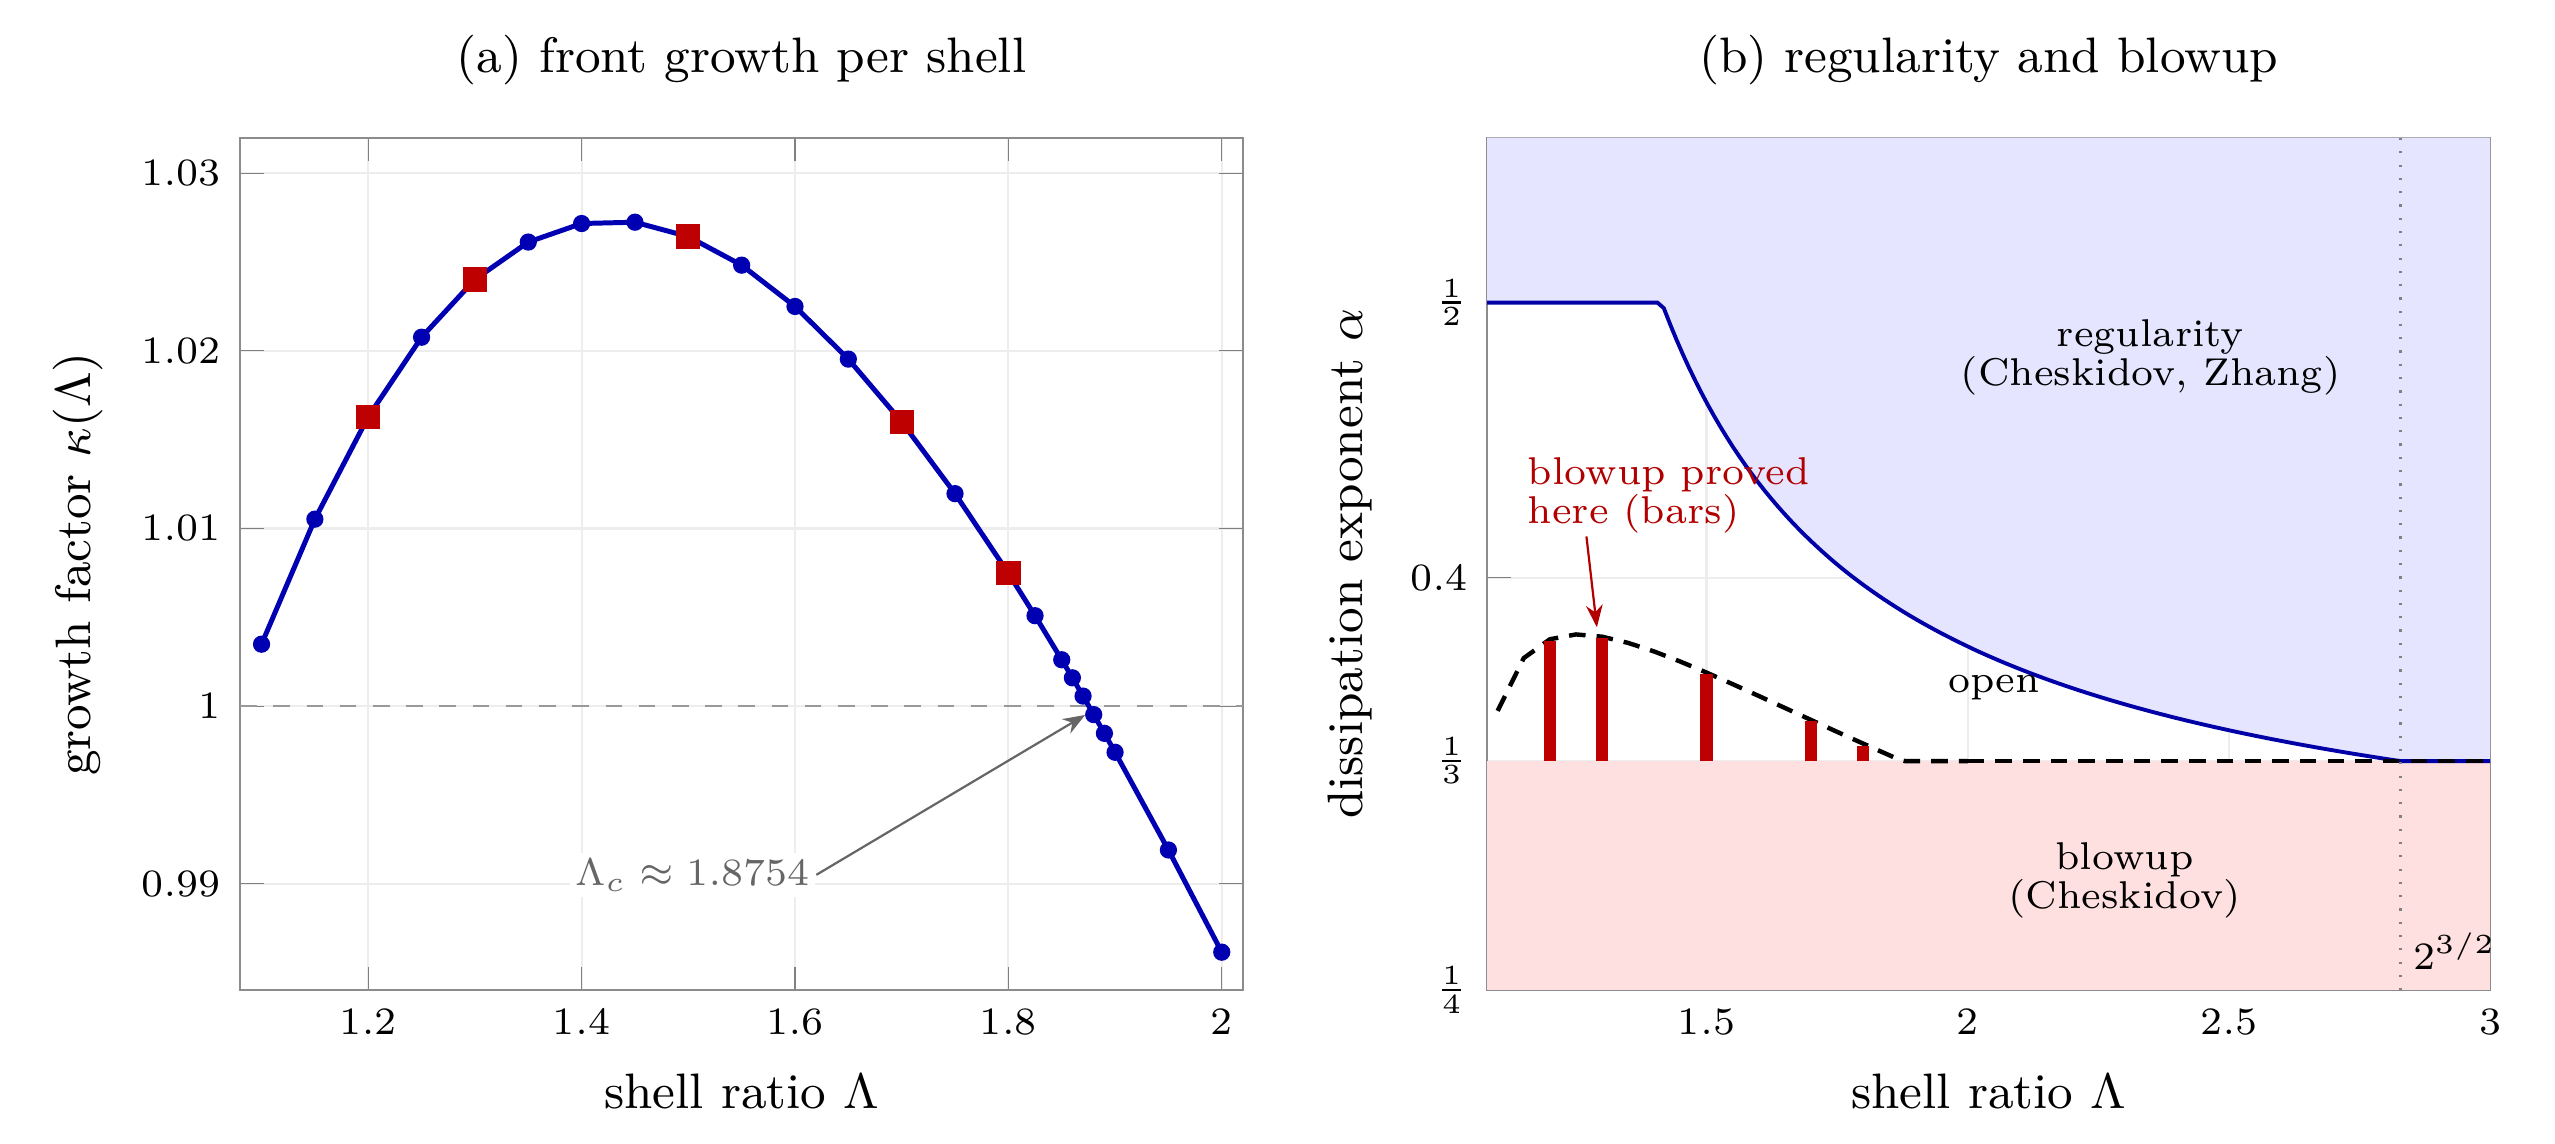
\includegraphics[width=\textwidth]{figures/fig_phase.png}
\caption{(a) The growth factor $\kappa(\Lambda)$ of the self-similar front
(Table~\ref{tab:kappa}); squares mark the five verified ratios. (b) Known
results in the $(\Lambda,\alpha)$ plane: blowup for $\alpha<1/3$ \cite{Che08};
regularity above $\min\{1/2,\max\{1/3,1/4+\log2/(8\log\Lambda)\}\}$
\cite{Che08,Zha26}; the bars are the ranges $[1/3,\alpha_\Lambda]$ proved here, and
the dashed curve is $\max\{1/3,\alpha^*(\Lambda)\}$.}
\label{fig:phase}
\end{figure}

The factor $\kappa(\Lambda)$ increases from $1$ near $\Lambda=1$ to a maximum
$1.0273$ near $\Lambda=1.42$, decreases, and crosses $1$ at
$\Lambda_c\approx1.8754$ (linear interpolation between $1.87$ and $1.88$). For
$\Lambda>\Lambda_c$ the fixed point has $\kappa<1$; a front from generic data then
does not follow it, and direct simulations of the inviscid model for
$\Lambda=1.9$, $2.2$, $2.5$, $3$ and $4$ show fronts with $\kappa=1$ to six
digits, that is, Kolmogorov scaling. Direct simulations of the viscous
model for $\Lambda=13/10$, started from the front profile, show growth of
$\Lambda^{(1-2\alpha)n}u_n$ over $900$ shells for $\alpha=0.36$, $0.37$, $0.375$ and decay for
$\alpha=0.385$, consistent with $\alpha^*(13/10)=0.3786$.

\begin{conjecture}\label{conj:threshold}
For $1<\Lambda<\Lambda_c$, the solutions with data near the front profile
lose regularity in finite time if and only if
$\alpha<\alpha^*(\Lambda)=1/3+\log\kappa(\Lambda)/(2\log\Lambda)$; for $\Lambda\ge\Lambda_c$ the
corresponding threshold is $1/3$.
\end{conjecture}

Theorem~\ref{thm:main} proves the ``if'' direction at five ratios, up to
the small gap between $\alpha_\Lambda$ and $\alpha^*(\Lambda)$ visible in Table~\ref{tab:main}.
The ``only if'' direction would require a regularity argument for $\alpha$
just above $\alpha^*(\Lambda)$, which is far beyond \eqref{eq:Zhang}: for $\Lambda=13/10$ the
known regularity starts at $\alpha=1/2$. Other data might blow up for
larger $\alpha$ through a different mechanism; we have no evidence either
way.

\section{Open questions}\label{sec:open}

\begin{enumerate}[label=(\arabic*)]
\item Prove Theorem~\ref{thm:main} for every $\Lambda$ in an interval, for
  instance by treating $\Lambda$ as an interval parameter. The verification
  is fast enough for a covering of $[1.1,1.85]$ by small intervals, but
  the window sizes $\Kb,\Ka$ must grow as $\Lambda\to1$ and the margin $\kappa-1$
  vanishes as $\Lambda\to\Lambda_c$.
\item Determine the threshold for $\Lambda\in[\Lambda_c,2^{3/2}]$, where
  Conjecture~\ref{conj:threshold} predicts $1/3$ and \eqref{eq:Zhang} gives
  regularity only above $1/4+\log2/(8\log\Lambda)$.
\item Prove regularity for some $\alpha<1/2$ when $\Lambda$ is small, or find
  blowup above $\alpha^*(\Lambda)$.
\item Explain the bifurcation at $\Lambda_c$, where the anomalous front meets
  the Kolmogorov front, in the language of the renormalization picture of
  \cite{Mai12,Mai13,DG98}.
\end{enumerate}

\appendix

\section{Code, data and checks}\label{app:code}

The repository \url{https://github.com/creelie/eNvrs}\zenodoline{}
\cite{Data} contains:
\begingroup\sloppy
\begin{itemize}
\item \texttt{cap/verify\_step.cpp}, \texttt{cap/MyHOE.h}: the verifier;
  \texttt{cap/run\_all.sh} builds it and runs the five cases;
  \texttt{cap/cases/}: profiles and radii; \texttt{cap/logs/}: the output,
  with all enclosures; \texttt{scripts/build\_capd.sh} builds the CAPD
  version used.
\item \texttt{crosscheck/recheck.py}: the interval re-check of the scalar
  inequalities; \texttt{crosscheck/front\_steps.c}: the C iteration of the
  full model; \texttt{crosscheck/kappa.jl}: the Julia computation of
  $\kappa(\Lambda)$; \texttt{numerics/}: the Python programs for the fixed point,
  Table~\ref{tab:kappa} and the simulations of Section~\ref{sec:numerics}.
\item \texttt{lean/DyadicNS.lean}: Lean~4 proofs, with Mathlib, of the
  induction in Lemma~\ref{lem:ahead}(b), the scalar case of
  Lemma~\ref{lem:deep}, the supersolution inequality in the proof of
  Lemma~\ref{lem:comparison}, the time estimate of
  Lemma~\ref{lem:section}(b), the monotonicity of $\eps_n$, the
  equivalence \eqref{eq:mech}, the summation of the step times and the
  divergence of the weighted amplitudes. Each theorem depends only on the
  axioms \texttt{propext}, \texttt{Classical.choice} and \texttt{Quot.sound}.
  The interval computation is not formalized.
\end{itemize}
\endgroup

\section*{Statements and declarations}

\noindent\textbf{Data availability.} All code, input files and output logs
are in the repository and its Zenodo archive \cite{Data}.

\noindent\textbf{Funding.} No funding was received for this work.

\noindent\textbf{Competing interests.} The author has no competing interests.

\noindent\textbf{Use of AI.} The computations, programs and drafting were
assisted by an AI system (Claude, Anthropic); the author checked the
mathematics and is responsible for the content.

\begin{thebibliography}{99}

\bibitem{BFM11} D.~Barbato, F.~Flandoli and F.~Morandin, Energy dissipation
and self-similar solutions for an unforced inviscid dyadic model,
\emph{Trans. Amer. Math. Soc.} \textbf{363} (2011), 1925--1946.
\href{https://doi.org/10.1090/S0002-9947-2010-05302-4}{doi:10.1090/S0002-9947-2010-05302-4}

\bibitem{BMR11} D.~Barbato, F.~Morandin and M.~Romito, Smooth solutions for
the dyadic model, \emph{Nonlinearity} \textbf{24} (2011), 3083--3097.
\href{https://doi.org/10.1088/0951-7715/24/11/004}{doi:10.1088/0951-7715/24/11/004}

\bibitem{Data} D.~Bhattacharjee, \emph{eNvrs: blowup above the exponent one
third in Katz--Pavlovi\'c dyadic models (code and data)}, GitHub
repository \url{https://github.com/creelie/eNvrs}, 2026, archived on Zenodo.

\bibitem{Che08} A.~Cheskidov, Blow-up in finite time for the dyadic model
of the Navier--Stokes equations, \emph{Trans. Amer. Math. Soc.}
\textbf{360} (2008), 5101--5120.
\href{https://doi.org/10.1090/S0002-9947-08-04494-2}{doi:10.1090/S0002-9947-08-04494-2}

\bibitem{CDF23} A.~Cheskidov, M.~Dai and S.~Friedlander, Dyadic models for
fluid equations: a survey, \emph{J. Math. Fluid Mech.} \textbf{25} (2023),
Paper No.~62.
\href{https://doi.org/10.1007/s00021-023-00799-3}{doi:10.1007/s00021-023-00799-3}

\bibitem{CFP07} A.~Cheskidov, S.~Friedlander and N.~Pavlovi\'c, Inviscid
dyadic model of turbulence: the fixed point and Onsager's conjecture,
\emph{J. Math. Phys.} \textbf{48} (2007), 065503.
\href{https://doi.org/10.1063/1.2395917}{doi:10.1063/1.2395917}

\bibitem{DG98} T.~Dombre and J.-L.~Gilson, Intermittency, chaos and
singular fluctuations in the mixed Obukhov--Novikov shell model of
turbulence, \emph{Phys. D} \textbf{111} (1998), 265--287.
\href{https://doi.org/10.1016/S0167-2789(97)80015-2}{doi:10.1016/S0167-2789(97)80015-2}

\bibitem{FP04} S.~Friedlander and N.~Pavlovi\'c, Blowup in a
three-dimensional vector model for the Euler equations, \emph{Comm. Pure
Appl. Math.} \textbf{57} (2004), 705--725.
\href{https://doi.org/10.1002/cpa.20017}{doi:10.1002/cpa.20017}

\bibitem{GS19} J.~G\'omez-Serrano, Computer-assisted proofs in PDE: a
survey, \emph{SeMA J.} \textbf{76} (2019), 459--484.
\href{https://doi.org/10.1007/s40324-019-00186-x}{doi:10.1007/s40324-019-00186-x}

\bibitem{Jeo19} I.-J.~Jeong, Self-similar solutions for dyadic models of
the Euler equations, \emph{J. Differential Equations} \textbf{266} (2019),
7197--7204.
\href{https://doi.org/10.1016/j.jde.2018.11.033}{doi:10.1016/j.jde.2018.11.033}

\bibitem{CAPD21} T.~Kapela, M.~Mrozek, D.~Wilczak and P.~Zgliczy\'nski,
CAPD::DynSys: a flexible C++ toolbox for rigorous numerical analysis of
dynamical systems, \emph{Commun. Nonlinear Sci. Numer. Simul.}
\textbf{101} (2021), 105578.
\href{https://doi.org/10.1016/j.cnsns.2020.105578}{doi:10.1016/j.cnsns.2020.105578}

\bibitem{KP05} N.~H.~Katz and N.~Pavlovi\'c, Finite time blow-up for a
dyadic model of the Euler equations, \emph{Trans. Amer. Math. Soc.}
\textbf{357} (2005), 695--708.
\href{https://doi.org/10.1090/S0002-9947-04-03532-9}{doi:10.1090/S0002-9947-04-03532-9}

\bibitem{KZ05} A.~Kiselev and A.~Zlato\v{s}, On discrete models of the
Euler equation, \emph{Int. Math. Res. Not.} \textbf{2005} (2005), no.~38,
2315--2339.
\href{https://doi.org/10.1155/IMRN.2005.2315}{doi:10.1155/IMRN.2005.2315}

\bibitem{Mai12} A.~A.~Mailybaev, Renormalization and universality of
blowup in hydrodynamic flows, \emph{Phys. Rev. E} \textbf{85} (2012),
066317.
\href{https://doi.org/10.1103/PhysRevE.85.066317}{doi:10.1103/PhysRevE.85.066317}

\bibitem{Mai13} A.~A.~Mailybaev, Bifurcations of blowup in inviscid shell
models of convective turbulence, \emph{Nonlinearity} \textbf{26} (2013),
1105--1124.
\href{https://doi.org/10.1088/0951-7715/26/4/1105}{doi:10.1088/0951-7715/26/4/1105}

\bibitem{Wal06} F.~Waleffe, On some dyadic models of the Euler equations,
\emph{Proc. Amer. Math. Soc.} \textbf{134} (2006), 2913--2922.
\href{https://doi.org/10.1090/S0002-9939-06-08293-1}{doi:10.1090/S0002-9939-06-08293-1}

\bibitem{Wal70} W.~Walter, \emph{Differential and Integral Inequalities},
Springer, Berlin, 1970.
\href{https://doi.org/10.1007/978-3-642-86405-6}{doi:10.1007/978-3-642-86405-6}

\bibitem{Zgl02} P.~Zgliczy\'nski, $C^1$ Lohner algorithm, \emph{Found.
Comput. Math.} \textbf{2} (2002), 429--465.
\href{https://doi.org/10.1007/s102080010025}{doi:10.1007/s102080010025}

\bibitem{Zha26} Z.~Zhang, Sharp regularity thresholds for viscous
Katz--Pavlovi\'c dyadic models, preprint (2026),
\href{https://arxiv.org/abs/2609.21312}{arXiv:2609.21312}.

\end{thebibliography}

\end{document}
